\chapter{\cookbookstitle: some useful examples}
\label{chapter:cookbooks}

The following cookbooks are provided as examples to facilitate the user configuring  \drexmtitle{}, \viztomotitle{} and \skstitle{} runs in different geodynamic model domains. The input parameter files (\texttt{*\_input.dat}) should be structured as provided, that is, preserving the same sequence of parameters. However, not all the parameters need to be considered, as some of them are only used when required (i.e., in 2D, the 3rd dimension is ignored; the size of the domain where to set a fossil fabric is considered only when \fonts{fossifabric} is > 0; visualization of the Lagrangian and Eulerian fields is active only when \fonts{Lagrangian} and \fonts{Eulerian} are > 0, respectively; etc.).\\  
In order to minimize the size of the \vtptitle{} files required to compute mantle fabrics, the examples below have been generated by low- to medium-resolution geodynamic models, and, in several cases, where the flow fields have reached or are assumed to have reached steady-state conditions.
For each cookbook, we provide parameter input files for software \drexmtitle{}, \viztomotitle{}, \vizvisctitle{} and \skstitle{}. \\
From each of the software directory execute:\\  

\drexmtitle{}: \texttt{./drexm ../cookbooks/DIRECTORY/drexm\_input.dat}

\viztomotitle{}: \texttt{./viztomo ../cookbooks/DIRECTORY/viztomo\_input.dat}

\vizvisctitle{}: \texttt{./vizvisc ../cookbooks/DIRECTORY/vizvisc\_input.dat} (provided only for \texttt{/2Dpolar\_convection})

\skstitle{}: \texttt{./calc\_split\_from\_flow\_model}\footnotemark


\footnotetext{Open the bash file \texttt{pbs\_sks}, and at lines 20 and 22 set, respectively, the directory \fonts{cijkl\_dir} (String) where the \cijkltitle{} file that you want to process is (and where the \texttt{stack\_input.dat} file has been copied), and its filenumber \fonts{timestep} (4 digit Integer)}

\vfill  % Fill the rest of the page with whitespace

\section{Steady-state convection in 2D cartesian coordinates}
\label{section:cookbook_2Dcartesianconvection}

\texttt{DIRECTORY: /2Dcartesian\_convection}

A 2D incompressible flow field in cartesian coordinates is given by the following analytical solution, whereby the radial and tangential velocities are: \\
\begin{center}
    $V_x(x,y) = -V_{x0}\sin(k_x2\pi/W)\cos(k_y\pi/H)$ \\
    $V_y(x,y) =  V_{y0}\cos(k_x2\pi/W)\sin(k_y\pi/H)$ \\
\end{center}

where $x$ and $y$ are the horizontal and vertical distance, $V_{x0}$ and $V_{y0}$ a constants, $k_x$ and $k_y$ are the horizontal and vertical wave numbers, $W$ and $H$ are the domain width and height. 

The \fonts{V} field is computed with the \matlabtitle{} script \texttt{cartesiancells.m} and saved to \texttt{vtp0001.h5} as a function of the numerical resolution, horizontal and vertical wave numbers. The model is mechanical, and thus  \fonts{ptmod = 0} in \texttt{drexm\_input.dat}.
The mantle fabrics computed with \drexmtitle{} in steady-state conditions for 5 Myr and visualized with \viztomotitle{} are shown in Fig. \ref{fig:cartesiancells}.


\begin{figure}[ht]
    \centering
    \includegraphics[width=1.0\textwidth]{cookbooks/2Dcartesian_convection_white.png}
    \caption{Steady-state convection pattern in cartesian coordinates created with \texttt{cartesiancells.m}. Radial anisotropy with superimposed Vp\textsubscript{max}.\\
    }
    \label{fig:cartesiancells}
\end{figure}

\vfill % Fill the rest of the page with whitespace

\section{Steady-state subduction in 2D polar coordinates}
\label{section:cookbook_2Dsubduction}

\texttt{DIRECTORY: /2Dpolar\_subduction}
\\
\\
Modeling the elastic properties in oceanic settings is fundamental to constrain the development of seismic anisotropy with formation, ageing and subduction of the oceanic lithosphere.\\  
Oceanic plate formation at the ridge and subsequent subduction at the trench is modelled in 2D polar coordinates with a modified version of the petrological-thermo-mechanical code \textbf{I2VIS} \citep{gerya2003pepi}. The domain is $(\phi,r)=(0-40^{\circ},5671-6371 km)$ and discretized with 1001x351 nodes, the ridge-trench distance is $25^{\circ}$, and a constant plate velocity of 4 cm/yr is imposed. 
The bottom boundary is open, and free slip is imposed on the other 3 boundaries. Free-surface is simulated with a 30 km thick air-layer.\\
The initial temperature field is defined by a constant temperature in the air layer (273 K), the half-space cooling model in the upper (20 Myr) and lower (0-62.5 Myr) plates, and a $0.5 K/km$ adiabat with a mantle potential temperature of $1540 K$.\\ 
The rheology is visco-plastic, and a composite low-T/diffusion/dislocation creep mechanism accommodates viscous deformation. Partial dry melting is simulated beneath the ridge according to parametrized solidus/liquidus curves (Fig. \ref{fig:meltviscosity}).\\ 

\begin{figure}
    \centering
    \includegraphics[width=0.9\textwidth]{EXEV/Melt+Viscosity.pdf}
    \caption{Close up of composition, melt fraction and viscosity (with superimposed the streamlines, white lines) of a 2D model of ridge dynamics and oceanic plate formation in polar coordinates.  
    }
    \label{fig:meltviscosity}
\end{figure}

The mantle fabrics are computed assuming steady-state conditions for 100 Myr, which is the time required by the crystal aggregates to move from the trench to the subduction zone, including the initial upwelling and final downwelling episodes.
The isoptropic P-wave distribution for an initial crystal aggregate spacing of 5 km is shown in Fig. \ref{fig:reflectreplicate} .\\

In order to check the role of melt-bearing cracks in seismic anisotropy, the mantle porosity has been saved in \texttt{dsd080melt.h5} and the SPO modelling has been activated in \texttt{viztomo\_input\_spo.dat} as shown in Fig. \ref{fig:extrinsic_anisotropy} for different SPO parameters defined in \texttt{\viztomotitle{}/spo\_input.dat}. 
By setting \fonts{spomod = 3} in \texttt{viztomo\_input.dat} and copying files \texttt{dsd080melt.h5} and \texttt{vtp0080.h5} in the output directory where the file \texttt{Cijkl0080.h5} is located, it is then possible to superimpose the effect of melt-bearing cracks on that due to LPO.


\begin{figure}
    \centering
    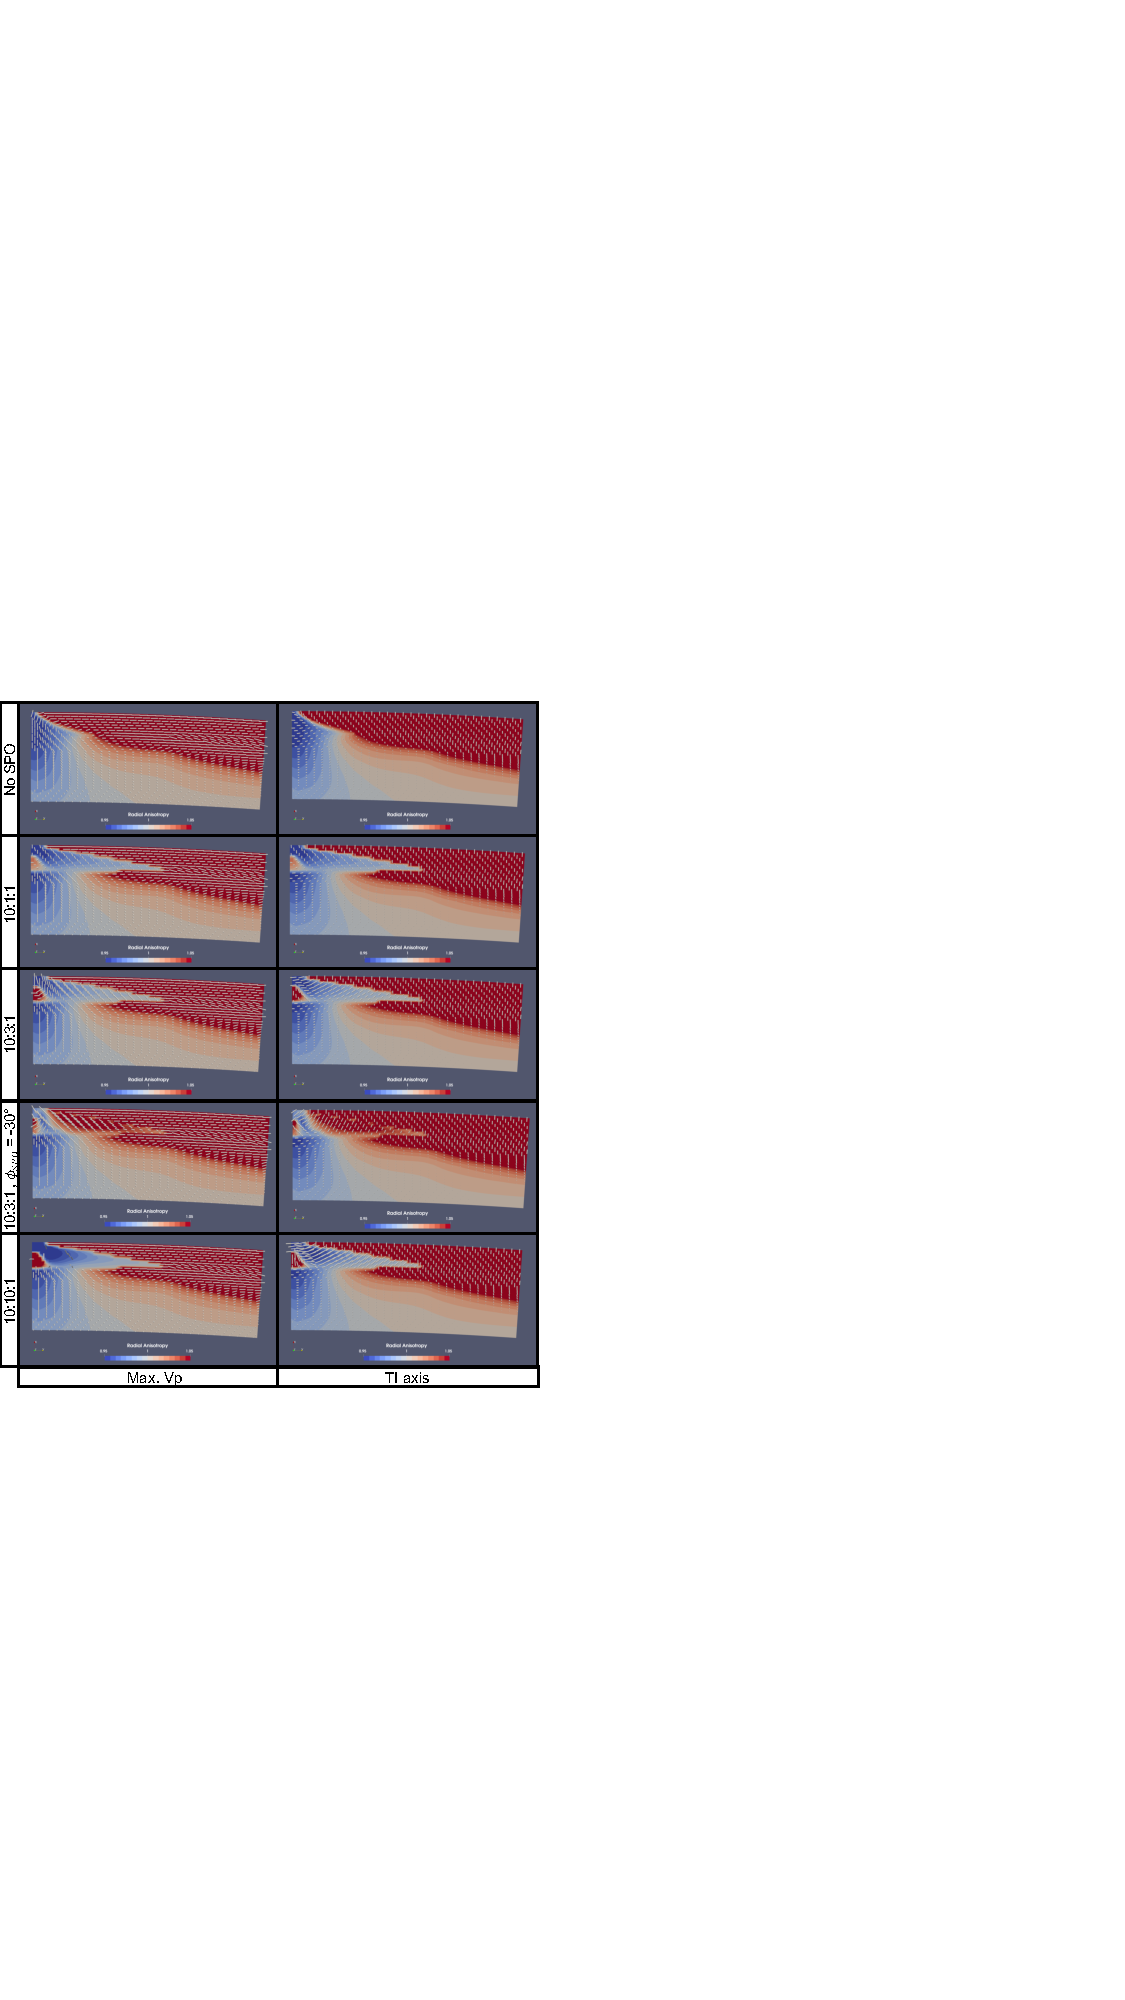
\includegraphics[width=0.9\textwidth]{EXEV/Anisotropy.pdf}
    \caption{Radial anisotropy with superimposed the orientation of Vp\textsubscript{max} (left) and TI axis (right) for the model in Fig. \ref{fig:meltviscosity}. In the top row the anisotropy is due to exclusively the strain-indcued LPO (AG-type olivine fabric) estimated with \drexmtitle{}, while in the underneath rows the LPO fabrics are superimposed with SPO fabrics due to the presence of melt. SPO control parameter used are \fonts{spomod = 3}; \fonts{meltspomod = 1}. The inclusions aspect ratio is indicated on the leftmost colums; \fonts{$\phi\textsubscript{SPO}$} is zero everywhere except in the second last row (-30$^{\circ}$). Note that for the penny-shaped inclusions (bottom row) the Vp\textsubscript{max} orientation is randomly oriented in the inclusion flat plane. The TI axis is normal to the flat inclusions, and parallel when cylindrical (second row).
    }
    \label{fig:extrinsic_anisotropy}
\end{figure}

\vfill % Fill the rest of the page with whitespace

\section{Steady-state global scale convection in 2D polar coordinates}
\label{section:cookbook_2Dconvection}

\texttt{DIRECTORY: /2Dpolar\_convection}

A 2D incompressible flow field in cylindrical coordinates is given by the following analytical solution, whereby the radial and tangential velocities are: \\
\begin{center}
    $V_r(\phi,r) = V_{r0}\cos(k_\phi\phi/2)\sin(k_r\pi r')$ \\
    $V_\phi(\phi,r) = -V_{\phi0}(r)\sin(k_\phi\phi/2)\cos(k_r\pi r')$ \\
    $V_{\phi0}(r) = 2V_{r0}/k_\phi[\tan(k_r\pi r') +  k_r\pi r/\Delta R )]$, \\
    $r' = (r - R_{min})/\Delta R$, \\
\end{center}

where $\phi$ and $r$ are longitude and radial distance, $V_{r0}$ a constant, $k_\phi$ and $k_r$ are the tangential and radial wave numbers, $\Delta R = R_{max} - R_{min}$, with $R_{min}$ and $R_{max}$ the bottom and top radial coordinate. 

Pressure distribution is:
\begin{center}
    $P(r) = P_0 + (R_{max} -r)/\Delta R \cdot P_1$ 
\end{center}
Temperature distribution is:
\begin{center}
    $T(\phi,r) = T_c(r) + dT (\phi,r)$

    $T_c(r) = T_0 + (R_{max} -r)/\Delta R \cdot T_1$

    $dT(\phi,r) = dT_{max}*V_r(\phi,r)/V_{r0}$
\end{center}
where $P_0$, $P_1$, $T_0$, $T_1$, $dT_{max}$, $V_{r0}$ are constants.

The \fonts{V}, \fonts{P} and \fonts{T} fields are computed with the \matlabtitle{} script \texttt{polarcells.m} and saved to \texttt{vtp0001.h5} as a function of the numerical resolution, radial and tangential wave numbers, and P-T conditions. 
The mantle fabrics computed with \drexmtitle{} in steady-state conditions for 100 Myr and visualized with \viztomotitle{} are shown in Fig. \ref{fig:polarcells} 
In global convection models, the vertical boundary should be open, i.e., the domain should be periodic along the tangential direction, thus:\\

    \begin{itemize}
        \item[] \fonts{dimensions = 2} 
        \item[] \fonts{cartspher = 2} 
        \item[] \fonts{x1periodic = 1} 
    \end{itemize}


\begin{figure}
    \centering
    \includegraphics[width=1.0\textwidth]{cookbooks/polarcells.pdf}
    \caption{Steady-state convection patterns in polar coordinates created with \texttt{polarcells.m}. A) P-wave velocity; B) S-wave velocity; C) Density; F) and I) Normalized P-P and P-S reflected energy; D) and E) P- and S-wave anomalies with respect horizonthally averaged velocities. G) Azimuthal anisotropy with superimposed fse\textsubscript{max}; H) Radial anisotropy with superimposed Vp\textsubscript{max}.\\
    }
    \label{fig:polarcells}
\end{figure}

\vfill % Fill the rest of the page with whitespace

\section{Sinking slab in 3D cartesian coordinates}
\label{section:cookbook_3Dcartesian_sinking}

\texttt{DIRECTORY: /3Dcartesian\_sinkingslab}

The flow field of a sinking cold horizontal slab is computed with the petrological-thermo-mechanical code \textbf{I3MG} \citep{gerya2003pepi}.
The domain is $(x,y,z)=(2000,1000,2000) km$ and discretized with 37x37x37 nodes, and free slip is imposed on all boundaries. The initial temperature field is defined by the half-space cooling model in the 90 km thick, 80 Myr old plate, a constant temperature of 473 K in the 100 km thick, 800 km long and 400 km wide slab centered with respect to the horizontal plane and initially at depth of 200-300 km, and a $0.5 K/km$ adiabat in the surrounding mantle with a potential temperature of $1540 K$. \\
The rheology is visco-plastic, and a composite low-T/diffusion/dislocation creep mechanism accounts for viscous deformation. An increase in viscosity is set at the 660 km depth discontinuity. \\

The mantle fabrics are computed using 20 \vtptitle files, for a total of 2 Myr. An initial (fossil) fabric is imposed on the horizontal slab with fast directions lying in the horizontal plane at $45^{\circ}$ from the x and z axes (Fig. \ref{fig:sinkinkslab_cartesian}.

\begin{figure}[ht]
    \centering
    \includegraphics[width=1.0\textwidth]{cookbooks/3Dcartesian_sinkingslab2.png}
    \caption{Time-dependent flow model of a sinking horizontal slab (contoured by the pink surface) in 3D cartesian coordinates. Radial anisotropy is shown on upper half of the image, while Vp\textsubscript{max} in the lower half. The white bars at the surface show SKS splitting, with length proportional to the delay time. The fossil fabric is shown by the orange bars close to the slab. Areas of sub-horizontal flow are characterized by positive radial anisotropy and sub-horizontal Vp\textsubscript{max}.\\
    }
    \label{fig:sinkinkslab_cartesian}
\end{figure}

\vfill % Fill the rest of the page with whitespace

\section{Sinking slab in 3D spherical coordinates}
\label{section:cookbook_3Dspherical_sinking}

\texttt{DIRECTORY: /3Dspherical\_sinkingslab}

An analogous model setup for the sinking slab in cartesian coordinates has been run in spherical coordinates using a modified version of \textbf{I3MG}. Differently form the previous example, the horizontal coordinates in the input files are now given in degrees rather in meters. The domain is $(\phi,r,\theta)=(80-100^{\circ},5371-6371 km,80-100^{\circ})$, and the slab is $8^{\circ}$ long and $4^{\circ}$ wide (Fig. \ref{fig:sinkinkslab_spherical}).
This model is used as an example for the seismic inversions performed with \syntomotitle{} (see \ref{SynTomo:Example}).

\begin{figure}[ht]
    \centering
    \includegraphics[width=1.0\textwidth]{cookbooks/3Dspherical_sinkingslab3.png}
    \caption{Time-dependent flow model of a sinking horizontal slab (contoured by the pink surface) similar to \ref{fig:sinkinkslab_cartesian} but in spherical coordinates.\\
    }
    \label{fig:sinkinkslab_spherical}
\end{figure}

\vfill % Fill the rest of the page with whitespace

\section{Steady-state global scale convection in 3D spherical coordinates}
\label{section:cookbook_3Dspherical_global}

\texttt{DIRECTORY: /3Dspherical\_global}

The global scale flow field has been simulated with a modified version of \textbf{I3MG} that solves the fundamental conservation equations of continuum mechanics in spherical coordinates using the Yin-Yang grid, an overset grid composed of to identical component grids that are combined in a complementary way to cover a spherical surface with partial overlap on their boundaries \citep{kageyama2004g3}. Each component grid is a low-latitude part of the latitude-longitude grid, and therefore the grid spacing is quasi-uniform. \\
The model is non-dimensional and discretized with 149x101x53x2 nodes, the initial temperature field is characterized by a conductive thermal gradient plus a thermal perturbation that varies along the radial direction with a sinusoidal pattern and laterally with cubic symmetry. The Rayleigh number is 14000, which yields a steady-state flow pattern.\\
In spherical coordinates, the mantle fabrics and their advection is computed by means of the Yin-Yang grid.  
The grids span over $-3\pi/4 -d\phi \leq \phi \leq 3\pi/4 + d\phi$ and $\pi/4 -d\theta \leq \theta \leq 3\pi/4  + d\theta$, where $d\phi$ and $d\theta$ are small buffers that ensure grids overlap, and usually taken equal to the grid spacing.\\
The longitudinal, radial and colatitudinal velocity components (in m/s or its adimensional counterpart), as well P,T and Fd, of the geodynamic model should then be interpolated to the nodes of the two grids as shown in the \matlabtitle{} script: \\
\texttt{/\drexmtitle/make\_HDF5\_vtp\_files/makevtpfiles\_yinyang.m}.\\
In global convection models, the vertical boundaries should be open, thus \fonts{x1periodic} and \fonts{x3periodic} must be set to $1$. As such, the Yin-Yang grid is activated in the \drexmtitle{} parameter input file by setting:
    \begin{itemize}
        \item[] \fonts{dimensions = 3} 
        \item[] \fonts{cartspher = 2} 
        \item[] \fonts{x1periodic = 1} 
        \item[] \fonts{x3periodic = 1}
    \end{itemize}

The \drexmtitle{} parameter input file is configured with adimensional \fonts{timemax} and distances, and such that the fabrics are computed only for upper mantle aggregates and without scaling the single crystal elastic tensors by the local P-T conditions. With an aggregate spacing of 80-90 km, about 1.3 millions of aggregates are distributed throughout the mantle, such that about 115 GB of memory needs to be allocated.
The azimuthal anisotropy related to these fabrics is shown in Fig. \ref{fig:globalconvection}, while the P-wave anomalies are shown in the manual cover image.

\begin{figure}[ht]
    \centering
    \includegraphics[width=1.0\textwidth]{cookbooks/3Dspherical_cubic2white.png}
    \caption{Steady-state global convection patterns in 3D spherical coordinates. The contours are T = 0.5. The bars indicate azimuthal anisotropy in the upper mantle.\\
    }
    \label{fig:globalconvection}
\end{figure}

\vfill % Fill the rest of the page with whitespace